% !TeX program = xelatex
\documentclass[a4paper,10pt]{article}

% ============================================================================
% កញ្ចប់បណ្ណាល័យ (Packages) – តាមលំនាំ NGS Preah Krasang (ls_plan.tex)
% បរិបទ៖ គ្មានស្លាយ LCD និងគ្មានម៉ាស៊ីនគិតលេខ — ប្រើសន្លឹកកិច្ចការសិស្ស (ស-ខ្មៅ) និងក្ដារខៀនជាគោល
% ============================================================================
\usepackage[a4paper, left=0.95cm, right=0.95cm, top=0.85cm, bottom=0.92cm, footskip=0.52cm]{geometry}
\usepackage{amsmath}
\usepackage{unicode-math}
\usepackage{fontspec}
\usepackage{array, longtable, multirow, colortbl}
\usepackage[table]{xcolor}
\usepackage{enumitem}
\usepackage{pifont}
\usepackage{fancyhdr}
\usepackage{tikz}
\usetikzlibrary{calc, arrows.meta, angles, quotes, decorations.markings, decorations.pathreplacing, patterns, babel}

\makeatletter
\let\@expl@@@mark@update@singlecol@structures@@\relax
\makeatother

\providecommand{\NGSFindFonts}{%
  \IfFileExists{C:/Windows/Fonts/cambria.ttc}{%
    \def\NGSSysPath{C:/Windows/Fonts/}%
    \def\NGSUserPath{C:/Users/KIT/AppData/Local/Microsoft/Windows/Fonts/}%
  }{%
    \IfFileExists{./fonts/KhmerOSsiemreap.ttf}{\def\NGSSysPath{./fonts/}\def\NGSUserPath{./fonts/}}{%
    \IfFileExists{../fonts/KhmerOSsiemreap.ttf}{\def\NGSSysPath{../fonts/}\def\NGSUserPath{../fonts/}}{%
    \IfFileExists{../../fonts/KhmerOSsiemreap.ttf}{\def\NGSSysPath{../../fonts/}\def\NGSUserPath{../../fonts/}}{%
    \IfFileExists{../../../fonts/KhmerOSsiemreap.ttf}{\def\NGSSysPath{../../../fonts/}\def\NGSUserPath{../../../fonts/}}{%
    \IfFileExists{../../../../fonts/KhmerOSsiemreap.ttf}{\def\NGSSysPath{../../../../fonts/}\def\NGSUserPath{../../../../fonts/}}{%
    \IfFileExists{../../../../../fonts/KhmerOSsiemreap.ttf}{\def\NGSSysPath{../../../../../fonts/}\def\NGSUserPath{../../../../../fonts/}}{%
    \IfFileExists{../../../../../../fonts/KhmerOSsiemreap.ttf}{\def\NGSSysPath{../../../../../../fonts/}\def\NGSUserPath{../../../../../../fonts/}}{%
      \def\NGSSysPath{../../../../../../../fonts/}\def\NGSUserPath{../../../../../../../fonts/}%
    }}}}}}}%
  }%
}
\NGSFindFonts

\setmathfont[Path={\NGSSysPath}, FontIndex=1, Scale=1.02]{cambria.ttc}
\defaultfontfeatures{Ligatures=TeX}

\setmainfont[
  Path={\NGSUserPath}, Extension=.ttf, Script=Khmer,
  BoldFont={KhmerOSsiemreap}, BoldFeatures={FakeBold=1.8},
  ItalicFont={KhmerOSsiemreap}, ItalicFeatures={FakeSlant=0.25},
  BoldItalicFont={KhmerOSsiemreap}, BoldItalicFeatures={FakeBold=1.8, FakeSlant=0.25}
]{KhmerOSsiemreap}

\newfontfamily\muol[Path={\NGSUserPath}, Extension=.ttf, Script=Khmer]{KhmerOSmuollight}
\newfontfamily\TimesEn[Path={\NGSSysPath}, Extension=.ttf, Scale=1.00, BoldFont={timesbd}, ItalicFont={timesi}, BoldItalicFont={timesbi}]{times}
\newfontfamily\NagaBold[Path={\NGSUserPath}, Extension=.ttf]{AKbalthom Naga Bold}
\newfontfamily\CalibriFont[Path={\NGSSysPath}, Extension=.ttf]{calibri}
\newfontfamily\Tacteing[Path={\NGSUserPath}]{TACTENG.TTF}
\newfontfamily\CourierBullet[Path={\NGSSysPath}, Extension=.ttf]{cour}
\newcommand{\wcirc}{{\CourierBullet\fontsize{9.5pt}{11pt}\selectfont o}}

\XeTeXlinebreaklocale "km"
\XeTeXlinebreakskip = 0pt plus 1pt minus 0.1pt

\definecolor{stepgray}{HTML}{D9D9D9}
\definecolor{headgray}{HTML}{F2F2F2}
\definecolor{boxgray}{HTML}{D9D9D9}
\definecolor{darkred}{HTML}{C00000}
\definecolor{red5e}{HTML}{FF0000}

\pagestyle{fancy}
\fancyhf{}
\renewcommand{\headrulewidth}{0pt}
\fancyfoot[R]{\CalibriFont\fontsize{11pt}{13pt}\selectfont\thepage}

\setlength{\parindent}{0pt}
\setlength{\parskip}{0pt}
\setlength{\tabcolsep}{3.8pt}

\newcolumntype{L}[1]{>{\raggedright\arraybackslash}p{#1}}
\newcolumntype{C}[1]{>{\centering\arraybackslash}p{#1}}

\newcommand{\en}[1]{{\TimesEn #1}}
\newcommand{\enbf}[1]{{\TimesEn\textbf{#1}}}
\newcommand{\unit}[1]{\,\text{\en{#1}}}
\newcommand{\fiveE}[1]{{\NagaBold\fontsize{9.5pt}{13pt}\selectfont\textcolor{red5e}{#1}}}
\newcommand{\timenote}[1]{\textcolor{darkred}{\textit{#1}}}
\newcommand{\redsub}[1]{\textcolor{darkred}{#1}}
\newcommand{\graybox}[1]{\colorbox{boxgray}{\strut\hspace{2pt}#1\hspace{2pt}}}
\newcommand{\ditem}{\tikz[baseline=-0.5ex]\fill (0,0.42ex) -- (0.42ex,0) -- (0,-0.42ex) -- (-0.42ex,0) -- cycle;\hspace{0.3em}}
\newcommand{\cnum}[1]{{\fontsize{10.5pt}{12pt}\selectfont\ding{\numexpr181+#1\relax}}\hspace{0.15em}}
\newcommand{\cfig}[1]{\par\vspace{3pt}{\centering #1\par}\vspace{3pt}}
\newcommand{\stepheader}[1]{\multicolumn{3}{|c|}{\cellcolor{stepgray}\muol #1} \\* \noalign{\hrule height 0.4pt}}
\newcommand{\khmflourish}{{\Tacteing\fontsize{36pt}{14pt}\selectfont\raisebox{-5pt}{3}}}

% ============================================================================
% ម៉ាក្រូគូសរូប TikZ ស-ខ្មៅ ១០០% សម្រាប់មេរៀន ២.៤.៦ (គ) ការគណនាឫសការេ (ROOT2)
% ============================================================================

% ១. E1 Engage: អន្ទាក់ក្បៀស \sqrt{153.76} និងការេប្រាកដ 2304 ទល់នឹង 2312
\newcommand{\figEngageROOTB}{%
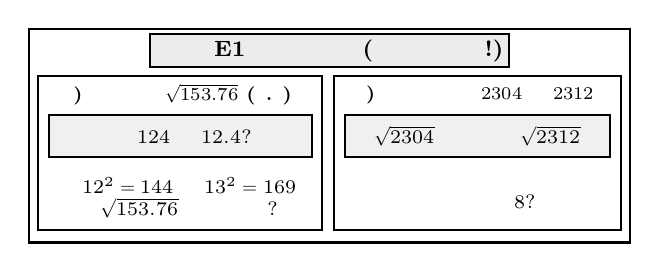
\begin{tikzpicture}[x=0.96cm, y=0.92cm, every node/.style={font=\scriptsize, text=black}]
  \draw[black, line width=0.95pt] (0,0) rectangle (7.95,2.95);
  \node[fill=gray!15, draw=black, line width=0.6pt, inner sep=2pt, font=\footnotesize\bfseries] at (3.975,2.65) {បេសកកម្ម \en{E1}៖ គណនាឫសការេដោយដៃ (គ្មានម៉ាស៊ីនគិតលេខ!)};

  \draw[black, line width=0.8pt] (0.12,0.18) rectangle (3.88,2.30);
  \node[font=\fontsize{6.6pt}{8.5pt}\selectfont\bfseries] at (2.00,2.04) {១) អន្ទាក់ក្បៀស៖ $\sqrt{153.76}$ (ទំ.២៤)};
  \draw[black, line width=0.75pt, fill=gray!12] (0.26,1.18) rectangle (3.74,1.76);
  \node at (2.00,1.47) {ស្មើ $124$ \;ឬ\; $12.4$?};
  \node[align=center] at (2.00,0.62) {បើ $12^2=144$ និង $13^2=169$\\តើ $\sqrt{153.76}$ ស្ថិតនៅចន្លោះណា?};

  \draw[black, line width=0.8pt] (4.04,0.18) rectangle (7.83,2.30);
  \node[font=\fontsize{6.5pt}{8.5pt}\selectfont\bfseries] at (5.935,2.04) {២) ពិនិត្យការេប្រាកដ៖ $2304$ និង $2312$};
  \draw[black, line width=0.75pt, fill=gray!12] (4.18,1.18) rectangle (7.69,1.76);
  \node at (5.935,1.47) {$\sqrt{2304}$ \quad ទល់នឹង \quad $\sqrt{2312}$};
  \node[align=center] at (5.935,0.62) {តើចំនួនមួយណាចេញពីឫសដាច់គត់\\ហើយមួយណាសល់សំណល់ $8$?};
\end{tikzpicture}}

% ២. E2 POE 1 & 2: យុទ្ធវិធីភ្លោះ លើ \sqrt{225} = 15 (ទំ.២៤)
\newcommand{\figTwinMethodROOTB}{%
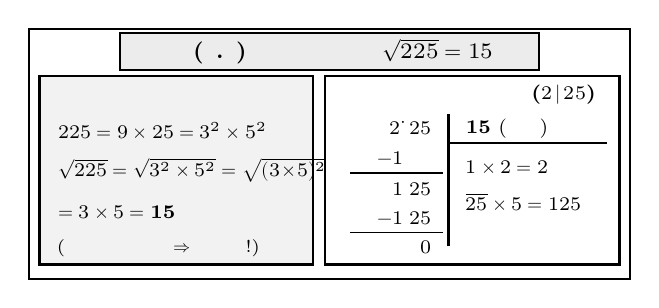
\begin{tikzpicture}[x=0.96cm, y=0.92cm, every node/.style={font=\scriptsize, text=black}]
  \draw[black, line width=0.95pt] (0,0) rectangle (7.95,3.45);
  \node[fill=gray!15, draw=black, line width=0.6pt, inner sep=2pt, font=\footnotesize\bfseries] at (3.975,3.14) {អនុវត្ត ១ (ទំ.២៤)៖ យុទ្ធវិធីភ្លោះគណនា $\sqrt{225} = 15$ ដោយដៃ};

  % Left: Method 1 Prime Factor Pairs
  \draw[black, line width=0.85pt, fill=gray!10] (0.14,0.20) rectangle (3.76,2.80);
  \node[font=\scriptsize\bfseries] at (1.95,2.54) {របៀបទី ១៖ បំបែកកត្តាបឋមជាគូ};
  \node[anchor=west] at (0.26,2.05) {$225 = 9 \times 25 = 3^2 \times 5^2$};
  \node[anchor=west] at (0.26,1.50) {$\sqrt{225} = \sqrt{3^2 \times 5^2} = \sqrt{(3\!\times\! 5)^2}$};
  \node[anchor=west] at (0.26,0.92) {$= 3 \times 5 = \mathbf{15}$};
  \node[anchor=west, font=\fontsize{6.2pt}{8pt}\selectfont] at (0.24,0.42) {(និទស្សន្តគូគ្រប់កត្តា $\Rightarrow$ ការេប្រាកដ!)};

  % Right: Method 2 Period Division
  \draw[black, line width=0.85pt] (3.92,0.20) rectangle (7.81,2.80);
  \node[font=\scriptsize\bfseries] at (5.865,2.54) {របៀបទី ២៖ វិធីចែកផ្ដាច់ពីរខ្ទង់ ($2\,|\,25$)};
  \draw[black, line width=0.8pt] (5.55,0.45) -- (5.55,2.28);
  \draw[black, line width=0.8pt] (5.55,1.88) -- (7.65,1.88);
  \node[anchor=east] at (5.45,2.08) {$2\,\dot{}\;25$};
  \node[anchor=east] at (5.45,1.66) {$-1\phantom{\;25}$};
  \draw[black, line width=0.6pt] (4.25,1.46) -- (5.48,1.46);
  \node[anchor=east] at (5.45,1.24) {$1\;25$};
  \node[anchor=east] at (5.45,0.84) {$-1\;25$};
  \draw[black, line width=0.6pt] (4.25,0.64) -- (5.48,0.64);
  \node[anchor=east] at (5.45,0.44) {$0$};
  % Right side of division bar
  \node[anchor=west] at (5.65,2.08) {$\mathbf{15}$ (ឫសការេ)};
  \node[anchor=west] at (5.65,1.54) {$1\times 2 = 2$};
  \node[anchor=west] at (5.65,1.06) {$\overline{25}\times 5 = 125$};
\end{tikzpicture}}

% ៣. E4 Decimal Period Division \sqrt{153.76} = 12.4
\newcommand{\figDecimalROOTB}{%
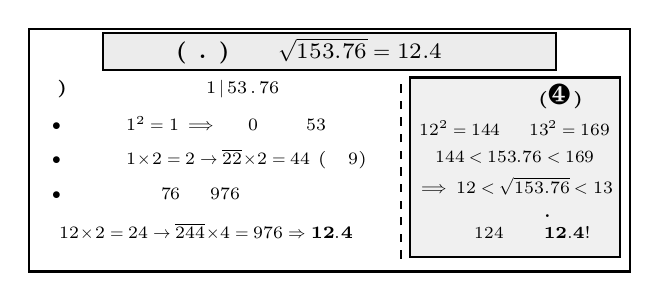
\begin{tikzpicture}[x=0.96cm, y=0.92cm, every node/.style={font=\scriptsize, text=black}]
  \draw[black, line width=0.95pt] (0,0) rectangle (7.95,3.35);
  \node[fill=gray!15, draw=black, line width=0.6pt, inner sep=2pt, font=\footnotesize\bfseries] at (3.975,3.04) {អនុវត្ត ២ (ទំ.២៤)៖ គណនា $\sqrt{153.76} = 12.4$ និងរបងប៉ាន់ស្មាន};

  % Left: Period division 1|53.|76
  \node[anchor=west, font=\fontsize{6.4pt}{8pt}\selectfont] at (0.18,2.52) {\textbf{១) ផ្ដាច់ពីរខ្ទង់ចេញពីក្បៀស៖} $1\,|\,53\,.\,76$};
  \node[anchor=west, font=\fontsize{6.3pt}{8pt}\selectfont] at (0.18,2.04) {$\bullet$ ខ្ទង់ទី ១៖ $1^2 = 1 \implies$ សល់ $0$ ទម្លាក់ $53$};
  \node[anchor=west, font=\fontsize{6.3pt}{8pt}\selectfont] at (0.18,1.56) {$\bullet$ ខ្ទង់ទី ២៖ $1\!\times\! 2=2 \to \overline{22}\!\times\! 2=44$ (សល់ $9$)};
  \node[anchor=west, font=\fontsize{6.3pt}{8pt}\selectfont] at (0.18,1.08) {$\bullet$ ឆ្លងក្បៀស ទម្លាក់ $76$ បាន $976$៖};
  \node[anchor=west, font=\fontsize{6.3pt}{8pt}\selectfont] at (0.28,0.56) {$12\!\times\! 2=24 \to \overline{244}\!\times\! 4 = 976 \Rightarrow \mathbf{12.4}$};

  \draw[black, dashed, line width=0.6pt] (4.92,0.18) -- (4.92,2.70);

  % Right: Magnitude Fence
  \draw[black, line width=0.8pt, fill=gray!12] (5.04,0.20) rectangle (7.82,2.68);
  \node[font=\fontsize{6.3pt}{8pt}\selectfont\bfseries] at (6.43,2.42) {របងប៉ាន់ស្មានទំហំ (\cnum{4})};
  \node[font=\fontsize{6.2pt}{8pt}\selectfont] at (6.43,1.98) {$12^2=144$ និង $13^2=169$};
  \node[font=\fontsize{6.2pt}{8pt}\selectfont] at (6.43,1.58) {$144 < 153.76 < 169$};
  \node[font=\fontsize{6.3pt}{8pt}\selectfont] at (6.43,1.18) {$\implies 12 < \sqrt{153.76} < 13$};
  \node[align=center, font=\fontsize{6.1pt}{7.6pt}\selectfont] at (6.43,0.62) {\textbf{កែតម្រូវពុម្ព ទំ.២៤៖}\\មិនមែន $124$ ទេ គឺ $\mathbf{12.4}$!};
\end{tikzpicture}}

% ៤. E5 Diagnostic Options A-D
\newcommand{\figExitCardsROOTB}{%
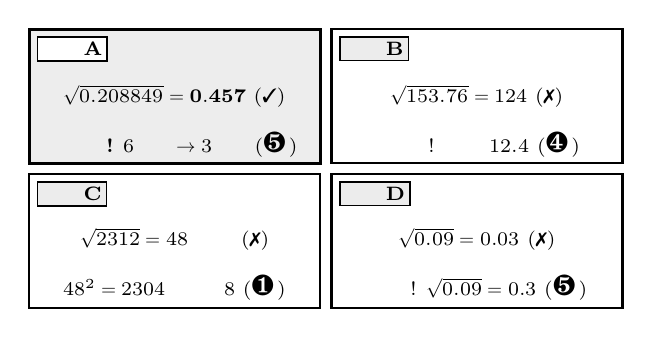
\begin{tikzpicture}[x=0.96cm, y=0.92cm, every node/.style={font=\scriptsize, text=black}]
  \draw[black, line width=1.1pt, fill=gray!14] (0,2.00) rectangle (3.85,3.85);
  \node[anchor=north west, fill=white, draw=black, line width=0.6pt, inner sep=1.8pt] at (0.10,3.75) {\textbf{ជម្រើស \en{A}}};
  \node at (1.925,2.92) {$\sqrt{0.208849} = \mathbf{0.457}$ (\ding{51})};
  \node at (1.925,2.25) {\textbf{ត្រឹមត្រូវ!} $6$ ខ្ទង់ $\to 3$ ខ្ទង់ (\cnum{5})};

  \draw[black, line width=0.9pt] (4.00,2.00) rectangle (7.85,3.85);
  \node[anchor=north west, fill=gray!15, draw=black, line width=0.6pt, inner sep=1.8pt] at (4.10,3.75) {\textbf{ជម្រើស \en{B}}};
  \node at (5.925,2.92) {$\sqrt{153.76} = 124$ (\ding{55})};
  \node at (5.925,2.25) {ភ្លេចក្បៀស! ត្រូវជា $12.4$ (\cnum{4})};

  \draw[black, line width=0.9pt] (0,0) rectangle (3.85,1.85);
  \node[anchor=north west, fill=gray!15, draw=black, line width=0.6pt, inner sep=1.8pt] at (0.10,1.75) {\textbf{ជម្រើស \en{C}}};
  \node at (1.925,0.95) {$\sqrt{2312} = 48$ ដាច់គត់ (\ding{55})};
  \node at (1.925,0.28) {$48^2=2304$ សល់សំណល់ $8$ (\cnum{1})};

  \draw[black, line width=0.9pt] (4.00,0) rectangle (7.85,1.85);
  \node[anchor=north west, fill=gray!15, draw=black, line width=0.6pt, inner sep=1.8pt] at (4.10,1.75) {\textbf{ជម្រើស \en{D}}};
  \node at (5.925,0.95) {$\sqrt{0.09} = 0.03$ (\ding{55})};
  \node at (5.925,0.28) {ខុសខ្ទង់! $\sqrt{0.09} = 0.3$ (\cnum{5})};
\end{tikzpicture}}

\begin{document}
\fontsize{10pt}{15.2pt}\selectfont

% -------------------- ក្បាលកិច្ចតែងការ --------------------
\begin{center}
  {\muol\fontsize{11pt}{16pt}\selectfont ព្រះរាជាណាចក្រកម្ពុជា}\\[2pt]
  {\muol\fontsize{10pt}{15pt}\selectfont ជាតិ សាសនា ព្រះមហាក្សត្រ}\\[1pt]
  \khmflourish
\end{center}

\vspace{-24pt}
{\muol\fontsize{9.5pt}{12.5pt}\selectfont
មន្ទីរអប់រំ យុវជន និងកីឡា ខេត្តកំពង់ធំ\\
ការិយាល័យអប់រំ យុវជន និងកីឡា ស្រុកកំពង់ស្វាយ\\
អនុវិទ្យាល័យព្រះក្រសាំង}

\vspace{1pt}
\begin{center}
  {\muol\fontsize{10pt}{14pt}\selectfont កិច្ចតែងការបង្រៀន}
\end{center}
\vspace{0pt}

% -------------------- ព័ត៌មានទូទៅ --------------------
{\renewcommand{\arraystretch}{0.98}
\hspace*{3.1cm}%
\begin{tabular}{@{}l l L{11.0cm}@{}}
  - \hspace{0.35cm} មុខវិជ្ជា & : & គណិតវិទ្យា ថ្នាក់ទី៨ (ពីជគណិត) \\
  - \hspace{0.35cm} ចំណងជើងមេរៀន & : & មេរៀនទី២៖ ស្វ័យគុណ \\
  - \hspace{0.35cm} ចំណងជើងរង & : & ៤.៦. គ. ការគណនាឫសការេ និងសំយោគមេរៀនទី២ (ទំ.២៤–២៦ លំហាត់ \#16–\#17) \\
  - \hspace{0.35cm} រយៈពេល & : & ១ ម៉ោងសិក្សា (៥០ នាទី) \\
  - \hspace{0.35cm} បង្រៀនដោយ & : & ហុក ប៊ុនថែន \\
  - \hspace{0.35cm} កាលបរិច្ឆេទ & : & ថ្ងៃសុក្រ ទី២០ ខែវិច្ឆិកា ឆ្នាំ២០២៦ \\
\end{tabular}

\vspace{2pt}

% -------------------- I. វត្ថុបំណង --------------------
\textbf{I.} {\muol វត្ថុបំណង}\\[1pt]
\hspace*{0.55cm}%
\begin{tabular}{@{}l l L{14.2cm}@{}}
  \wcirc \hspace{0.25cm} វិជ្ជាសម្បទា & : & សិស្សប្រាប់វិធីទាំងពីរក្នុងការគណនាឫសការេដោយដៃ គឺការបំបែកកត្តាបឋមជាគូ និងវិធីចែកផ្ដាច់ពីរខ្ទង់ចេញពីក្បៀសទសភាគ ព្រមទាំងក្បួនប៉ាន់ស្មានទំហំឫសការេ ។ \\
  \wcirc \hspace{0.25cm} បំណិនសម្បទា & : & សិស្សគណនាឫសការេនៃចំនួនគត់ ទសភាគ និងប្រភាគ (ទំ.២៤ និង ទំ.២៦ \#16–\#17) ដោយដៃលើសន្លឹកកិច្ចការ ដោយមិនប្រើម៉ាស៊ីនគិតលេខ និងសំយោគច្បាប់សំខាន់ៗនៃមេរៀនទី២ ។ \\
  \wcirc \hspace{0.25cm} ចរិយាសម្បទា & : & សិស្សមានទម្លាប់ផ្ទៀងផ្ទាត់តម្លៃឫសការេដោយរបងប៉ាន់ស្មានទំហំ ($k^2 < N < (k+1)^2$) និងមានទំនុកចិត្តលើការគណនាដោយដៃ ។ \\
\end{tabular}

\vspace{2pt}

% -------------------- II. សម្ភារៈឧបទេស --------------------
\textbf{II.} {\muol សម្ភារៈឧបទេស}\\[1pt]
\hspace*{0.55cm}$\bullet$ \hspace{0.35cm} សៀវភៅសិក្សាគោលគណិតវិទ្យាថ្នាក់ទី៨ (ទំ.២៤–២៦) ក្ដារខៀន ដីស និងសន្លឹកកិច្ចការសិស្ស ស-ខ្មៅ (\en{Worksheet\_ROOT2} ទំព័រ ១–២ សម្រាប់បំពេញផ្ទាល់ គ្មានស្លាយ \en{LCD} និងគ្មានម៉ាស៊ីនគិតលេខ)

\vspace{2pt}

% -------------------- III. វិធីសាស្រ្តបង្រៀន --------------------
\textbf{III.} {\muol វិធីសាស្រ្តបង្រៀន}\\[1pt]
\hspace*{0.45cm}%
\begin{tabular}{@{}l l L{14.85cm}@{}}
  $\bullet$ \hspace{0.25cm} គោលវិធី & : & សិស្សមជ្ឈមណ្ឌល (បង្រៀនតាមសន្លឹកកិច្ចការស៊ើបអង្កេត និងក្ដារខៀន គ្មាន \en{LCD}) \\
  $\bullet$ \hspace{0.25cm} យុទ្ធវិធីបង្រៀន & : & គំរូ \en{5Es} រួមបញ្ចូលយុទ្ធវិធីភ្លោះ បំបែកកត្តាបឋមជាគូ ទល់នឹង វិធីចែកផ្ដាច់ពីរខ្ទង់ និងរបងប៉ាន់ស្មានទំហំ (\en{Magnitude Bounding Fence}) \\
\end{tabular}
}

\vspace{2pt}

% -------------------- IV. ដំណើរការបង្រៀន --------------------
\textbf{IV.} {\muol ដំណើរការបង្រៀន}

\vspace{1pt}

\renewcommand{\arraystretch}{1.15}
\begin{longtable}{|L{5.50cm}|L{7.90cm}|L{4.80cm}|}
\hline
\rowcolor{headgray}
\multicolumn{1}{|c|}{\muol សកម្មភាពគ្រូ} &
\multicolumn{1}{c|}{\muol ខ្លឹមសារមេរៀន} &
\multicolumn{1}{c|}{\muol សកម្មភាពសិស្ស} \\
\hline
\endfirsthead
\hline
\endhead
\hline
\endfoot
\hline
\endlastfoot

% ==================== ជំហានទី១ (2min) ====================
\stepheader{ជំហានទី១ \enbf{(}រដ្ឋបាលថ្នាក់\enbf{)}}
$\bullet$ ពិនិត្យអវត្តមាន អនាម័យ និងសណ្ដាប់ធ្នាប់ថ្នាក់រៀន
&
$\bullet$ រដ្ឋបាលថ្នាក់ និងការរៀបចំដៃគូសិក្សា
&
$\circ$ ប្រធានថ្នាក់រាយការណ៍អវត្តមាន \\[3pt]

$\bullet$ ចែក \textbf{សន្លឹកកិច្ចការសិស្ស (\en{Worksheet\_ROOT2})} ម្នាក់ ១ សន្លឹក (ផ្កាប់ទុកសិន)
&
$\bullet$ សន្លឹកកិច្ចការសិស្ស ស-ខ្មៅ (\en{Worksheet\_ROOT2} ទំព័រ ១–២)
&
$\circ$ ទទួលសន្លឹកកិច្ចការ និងត្រៀមសម្ភារៈសរសេរ \\
\hline

% ==================== ជំហានទី២ (9min: <=3 + 3 + E1 3) ====================
\stepheader{ជំហានទី២ \enbf{(}កិច្ចការផ្ទះ \enbf{+} ទំនាក់ទំនងមេរៀនថ្មី\enbf{)}}
\ditem \textbf{កំណែកិច្ចការផ្ទះ ($\le 3\unit{min}$)} \timenote{(កុំសរសេរវែង)} \par
$\bullet$ ហៅសិស្ស ២ នាក់ឡើងសរសេរចម្លើយលំហាត់ \#12, \#13 និង \#15 (ទំ.២៦) លើក្ដារខៀន
&
{\centering\redsub{កំណែកិច្ចការផ្ទះមេរៀន ៤.៦ ក, ខ (ទំ.២៦ \#12–\#15)}\par} \par
$\bullet$ \textbf{\#12៖} $9\unit{cm},\; 0.2\unit{m},\; \frac{4}{5}\unit{dm}$ \;;\; \textbf{\#13៖} $\pm 6,\; \pm 11,\; \pm 1.2$, គ្មានឫស \par
$\bullet$ \textbf{\#14៖} $4,\; -5,\; 0.2$ \;;\; \textbf{\#15៖} $x = \sqrt[3]{216} = 6\unit{cm}$
&
$\circ$ ផ្ទៀងផ្ទាត់ចម្លើយក្នុងសៀវភៅកិច្ចការផ្ទះ \\[3pt]

\ditem \textbf{រំលឹកមេរៀនទាក់ទង (3min)} \par
$\bullet$ សួររហ័ស៖ បំបែក $36$ ជាផលគុណកត្តាបឋម និងគណនា $10^2, 12^2, 13^2, 20^2, 50^2$
&
{\centering\redsub{រំលឹកកត្តាបឋម និងការេគោលសម្រាប់ប៉ាន់ស្មាន}\par} \par
$\bullet$ $36 = 2^2 \times 3^2 = (2\times 3)^2 \implies \sqrt{36} = 2\times 3 = 6$ \par
$\bullet$ $10^2 = 100,\; 12^2 = 144,\; 13^2 = 169,\; 20^2 = 400,\; 50^2 = 2500$
&
$\circ$ ឆ្លើយរហ័សអំពីការបំបែកកត្តាបឋម និងការេគោល \\[3pt]

\fiveE{E1 - Engage (3min)} \timenote{(កុំទាន់ផ្ដល់ចម្លើយ)} \par
\ditem \textbf{«បេសកកម្មគ្មានម៉ាស៊ីនគិតលេខ៖ ចាប់កំហុសក្បៀស និងការេមិនប្រាកដ!»} \par
$\bullet$ ឱ្យសិស្សបើកសន្លឹកកិច្ចការទំព័រ ១ គូសធីកទស្សន៍ទាយលើសំណួរ ២
&
{\centering\redsub{បេសកកម្ម E1៖ អន្ទាក់ $\sqrt{153.76}$ និង $2304$ ទល់នឹង $2312$}\par} \par
$\bullet$ \textbf{សំណួរ ១៖} តើ $\sqrt{153.76}$ ស្មើ $124$ (ដូចបោះពុម្ពទំ.២៤) ឬស្មើ $12.4$? \par
$\bullet$ \textbf{សំណួរ ២៖} រវាង $2304$ និង $2312$ តើមួយណាជាការេប្រាកដ ($\sqrt{\phantom{x}}=48$) ហើយមួយណាសល់សំណល់ $8$?
&
$\circ$ គូសធីកទស្សន៍ទាយលើសន្លឹកកិច្ចការទំព័រ ១ \\[3pt]

&
\cfig{\figEngageROOTB}
& \\[3pt]

$\bullet$ ស្រង់ចំនួនដៃសិស្សកត់លើក្ដារខៀន (មិនទាន់ប្រាប់ចម្លើយត្រូវ)
&
$\bullet$ ស្ថិតិទស្សន៍ទាយ៖ $124$ ទល់នឹង $12.4$ ; $2304$ ទល់នឹង $2312$
&
$\circ$ លើកដៃបង្ហាញការទស្សន៍ទាយ \\
\hline

% ==================== ជំហានទី៣ (17min: E2 11m + E3 6m) ====================
\stepheader{ជំហានទី៣ \enbf{(}ខ្លឹមសារមេរៀនថ្មី\enbf{)}}
\fiveE{E2 - Explore (11min)} \par
$\bullet$ សរសេរចំណងជើងរងលើក្ដារខៀន
&
\textbf{៤.៦. គ. ការគណនាឫសការេ និងសំយោគមេរៀនទី២} (ទំ.២៤–២៥)
&
$\circ$ កត់ចំណងជើងចូលសៀវភៅ \\[3pt]

\ditem \textbf{សកម្មភាព ១៖ បំបែកកត្តាបឋមជាគូ \en{POE 1} (5min, ទំ.២៤ ផ្នែកទី១-ក)} \par
$\bullet$ ឱ្យដៃគូបំបែក $225$ និង $625$ ជាផលគុណកត្តាបឋម រួចផ្គុំជាគូការេលើសន្លឹកកិច្ចការ
&
{\centering\textbf{សកម្មភាព ១ (\en{POE 1})៖ របៀបទី ១ — បំបែកកត្តាបឋមជាគូ}\par} \par
$\bullet$ $\sqrt{225} = \sqrt{3^2\times 5^2} = 3\times 5 = \mathbf{15}$ \par
$\bullet$ $\sqrt{625} = \sqrt{5^4} = \sqrt{(5^2)^2} = 5^2 = \mathbf{25}$
&
$\circ$ បំបែកកត្តាបឋម និងទាញកត្តាម្ដងមួយចេញពីគូការេនីមួយៗ \\[3pt]

\ditem \textbf{សកម្មភាព ២៖ វិធីចែកផ្ដាច់ពីរខ្ទង់ពីស្ដាំទៅឆ្វេង \en{POE 2} (6min, ទំ.២៤ ផ្នែកទី១-ខ)} \par
$\bullet$ ដឹកនាំដៃគូអនុវត្តវិធីចែកផ្ដាច់ពីរខ្ទង់លើ $2\,|\,25$ និង $6\,|\,25$ តាមគំរូអនុវត្ត ១ (ទំ.២៤)
&
{\centering\textbf{សកម្មភាព ២ (\en{POE 2})៖ របៀបទី ២ — វិធីចែកផ្ដាច់ពីរខ្ទង់}\par} \par
$\bullet$ ផ្ដាច់ $2\,|\,25$៖ $1^2=1$ (សល់ $1$), ទម្លាក់ $25$ បាន $125$ \par
$\bullet$ យកឫស $1\times 2 = 2$ រួចដាក់លេខ $5$៖ $\overline{25}\times 5 = 125 \implies \sqrt{225} = \mathbf{15}$
&
$\circ$ បំពេញប្រអប់វិធីចែកផ្ដាច់ពីរខ្ទង់លើ $\sqrt{225}$ និង $\sqrt{625}$ \\[3pt]

&
\cfig{\figTwinMethodROOTB}
& \\[3pt]

% --- E3 Explain (6min) ---
\fiveE{E3 - Explain (6min)} \par
\ditem \textbf{បង្គុំក្បួនគណនាឫសការេដោយដៃ និងធនាគារហេតុផល (ផ្នែកទី២)} \par
$\bullet$ សំយោគក្បួនទាំង ២ និងភ្ជាប់ទៅប្រអប់សង្ខេបមេរៀនទី២ (ទំ.២៥)
&
$\bullet$ \textbf{ក្បួនសំយោគ (ទំ.២៤–២៥)៖} គេអាចគណនាឫសការេដោយដៃតាម៖ (១) \textbf{បំបែកកត្តាបឋមជាគូ} ($\sqrt{a^2 b^2}=ab$) ឬ (២) \textbf{វិធីចែកផ្ដាច់ពីរខ្ទង់ចេញពីក្បៀសទសភាគ} រួមជាមួយរបងប៉ាន់ស្មានទំហំ ។
&
$\circ$ បំពេញប្រអប់សំយោគលើសន្លឹកកិច្ចការ \\[3pt]

$\bullet$ សង្ខេប \textbf{ធនាគារហេតុផល \cnum{1}--\cnum{3}} សម្រាប់ការបំបែកកត្តាបឋម និងវិធីចែកផ្ដាច់ពីរខ្ទង់
&
\textbf{ធនាគារហេតុផល \en{B\&W} (\cnum{1}--\cnum{5})៖} \par
\cnum{1} បំបែកកត្តាបឋមជាគូ៖ $\sqrt{p^{2k} q^{2m}} = p^k q^m$ (បើសល់និទស្សន្តសេស មិនមែនការេប្រាកដទេ) \par
\cnum{2} ផ្ដាច់ពីរខ្ទង់៖ ផ្ដាច់ពីរខ្ទង់ម្ដងចេញពីក្បៀសទសភាគ (ទៅឆ្វេង និងទៅស្ដាំ) \par
\cnum{3} គុណឫសនឹង $2$៖ យកឫសរកឃើញ $a$ គុណនឹង $2$ រកលេខ $b$ ដែល $\overline{(2a)b}\times b \le$ សំណល់
&
$\circ$ ផ្ទៀងផ្ទាត់ហេតុផល \cnum{1}--\cnum{3} លើសន្លឹកកិច្ចការ \\[3pt]

$\bullet$ សង្ខេប \textbf{ធនាគារហេតុផល \cnum{4}--\cnum{5}} សម្រាប់របងប៉ាន់ស្មាន ទសភាគ និងប្រភាគ
&
\cnum{4} របងប៉ាន់ស្មានទំហំ៖ បើ $k^2 < N < (k+1)^2 \implies k < \sqrt{N} < k+1$ (ការពារច្រឡំក្បៀស!) \par
\cnum{5} ប្រភាគ និងទសភាគ៖ $\sqrt{\frac{a}{b}} = \frac{\sqrt{a}}{\sqrt{b}}$ ; ចំនួនខ្ទង់ទសភាគរបស់ $\sqrt{N}$ ស្មើពាក់កណ្ដាលនៃ $N$
&
$\circ$ ផ្ទៀងផ្ទាត់ហេតុផល \cnum{4}--\cnum{5} លើសន្លឹកកិច្ចការ \\
\hline

% ==================== ជំហានទី៤ (20min: E4 10m + E5 10m) ====================
\stepheader{ជំហានទី៤ \enbf{(}ពង្រីកចំណេះដឹង និងវាយតម្លៃ\enbf{)}}
\fiveE{E4 - Elaborate (10min)} \par
\ditem \textbf{អនុវត្ត ២ និងការកែតម្រូវកំហុសពុម្ពទំ.២៤ (សន្លឹកកិច្ចការ ទំព័រ ២ ផ្នែកទី៣)} \par
$\bullet$ ដឹកនាំគណនាដោយដៃលើ \textbf{អនុវត្ត ២ ($\sqrt{529}$ និង $\sqrt{153.76}$ — ទំ.២៤)}
&
{\muol លំហាត់គំរូ} \textbf{(អនុវត្ត ២ និងការផ្ទៀងផ្ទាត់ ទំ.២៤)៖} \par
$\bullet$ \textbf{ក.} $\sqrt{529}$ ($5\,|\,29$)៖ $2^2=4$ (សល់ $129$), $2\times 2=4 \to \overline{43}\times 3=129 \implies \mathbf{23}$ (\cnum{2}, \cnum{3}) \par
$\bullet$ \textbf{ខ.} $\sqrt{153.76}$ ($1\,|\,53\,.\,76$)៖ ដោយ $12^2=144 < 153.76 < 169=13^2$ និងវិធីចែកផ្ដាច់ពីរខ្ទង់ បាន $\mathbf{12.4}$ \timenote{(កែតម្រូវពុម្ពទំ.២៤ ដែលដាក់ $124$!)} (\cnum{4})
&
$\circ$ អនុវត្តវិធីចែកផ្ដាច់ពីរខ្ទង់លើសន្លឹកកិច្ចការ និងកត់ចំណាំកែតម្រូវលើសៀវភៅពុម្ព ទំ.២៤ \\[3pt]

$\bullet$ ដឹកនាំពិនិត្យភាពខុសគ្នារវាងការេប្រាកដ $2304$ និងការេមិនប្រាកដ $2312$ (ទំ.២៤)
&
$\bullet$ \textbf{គ.} $\sqrt{2304} = \mathbf{48}$ ដាច់គត់ ឯ $2312 = 48^2 + 8 = 2^3\times 17^2$ សល់សំណល់ $8$! (\cnum{1})
&
$\circ$ កត់សម្គាល់ការពិនិត្យសំណល់ និងនិទស្សន្តកត្តាបឋម \\[3pt]

&
\cfig{\figDecimalROOTB}
& \\[3pt]

$\bullet$ សួរសំណួរឆ្លុះបញ្ចាំង \textbf{\en{EIA Looking-Back} (៣០ វិនាទី)}
&
\textbf{\en{EIA Looking-Back}៖} «បើទសភាគ $0.208849$ មាន $6$ ខ្ទង់ក្រោយក្បៀស តើ $\sqrt{0.208849}$ ត្រូវមានប៉ុន្មានខ្ទង់ក្រោយក្បៀស?»
&
$\circ$ ឆ្លើយ៖ «ត្រូវមាន $6\div 2 = 3$ ខ្ទង់ក្រោយក្បៀស ($\to 0.457$)!» \\[3pt]

% --- E5 Evaluate (10min) ---
\fiveE{E5 - Evaluate (10min)} \par
\ditem \textbf{ហ្វឹកហាត់ជាដៃគូលើ «ប្រតិបត្តិ ២» (6min, ទំ.២៤ — ផ្នែកទី៤-ក)} \par
$\bullet$ ឱ្យដៃគូគណនាដោយដៃលើ \textbf{ប្រតិបត្តិ ២ ក និង ខ (ទំ.២៤)}
&
{\muol លំហាត់ប្រតិបត្តិ} \textbf{(ទំ.២៤ — គណនាដោយដៃ ១០០\%)៖} \par
$\bullet$ \textbf{ក.} $\sqrt{3249}$ ($32\,|\,49$)៖ $5^2=25$ (សល់ $749$), $\overline{107}\times 7 = 749 \implies \mathbf{57}$ (\cnum{2}, \cnum{3}) \par
$\bullet$ \textbf{ខ.} $\sqrt{0.208849}$ ($0.\,20\,|\,88\,|\,49$)៖ $4^2=16$, $\overline{85}\times 5=425$, $\overline{907}\times 7=6349 \implies \mathbf{0.457}$ (\cnum{5})
&
$\circ$ គណនាប្រតិបត្តិ ក និង ខ ដោយដៃលើសន្លឹកកិច្ចការ \\[3pt]

$\bullet$ ឱ្យដៃគូគណនាបន្តលើ \textbf{ប្រតិបត្តិ ២ គ និង ឃ} រួចប្ដូរសន្លឹកផ្ទៀង (\en{Pause-Review})
&
$\bullet$ \textbf{គ.} $\sqrt{\dfrac{2025}{169}} = \dfrac{\sqrt{2025}}{\sqrt{169}} = \dfrac{\mathbf{45}}{\mathbf{13}}$ (\cnum{5}) \;;\; \textbf{ឃ.} $\sqrt{1225} = \sqrt{5^2\times 7^2} = \mathbf{35}$ (\cnum{1})
&
$\circ$ គណនាប្រតិបត្តិ គ និង ឃ រួចប្ដូរសន្លឹកផ្ទៀងជាមួយដៃគូ \\[3pt]

$\bullet$ បិទបេសកកម្ម \en{E1} និងឱ្យសិស្សវិនិច្ឆ័យ \textbf{ជម្រើស \en{A--D}} + \textbf{\en{Exit Check}} (4min)
&
$\bullet$ \textbf{បិទបេសកកម្ម \en{E1}៖} $\sqrt{153.76} = 12.4$ ; $\sqrt{2304} = 48$ ដាច់គត់ ឯ $2312$ សល់សំណល់ $8$ ។ \par
$\bullet$ \textbf{វិនិច្ឆ័យជម្រើស \en{A--D} លើសន្លឹកកិច្ចការ៖}
&
$\circ$ ផ្ទៀងចម្លើយ \en{E1} និងគូសវង់ជម្រើសត្រូវ \en{A} \\[3pt]

&
\cfig{\figExitCardsROOTB}
& \\[3pt]

$\bullet$ ពិនិត្យរហ័សលើសំបុត្រចេញសំយោគមេរៀនទី២ នៅបាតសន្លឹកកិច្ចការ (៦០ វិនាទី)
&
$\bullet$ \textbf{\en{Exit Check} (សំយោគមេរៀនទី២)៖} ១) $\sqrt{625} = 25$ ; ២) $\sqrt{1.44} = 1.2$ ; ៣) $0.0004 = 4\times 10^{-4}$ ។
&
$\circ$ បំពេញសំបុត្រចេញទាំង ៣ ខ្ទង់ដោយខ្លួនឯង \\
\hline

% ==================== ជំហានទី៥ (<=2min) ====================
\stepheader{ជំហានទី៥ \enbf{(}កិច្ចការផ្ទះ \enbf{+} បណ្ដាំផ្ញើ\enbf{)}}
\timenote{ចំណាយពេលឱ្យតិចបំផុតកុំឱ្យលើស 2min} \par
$\bullet$ ណែនាំកិច្ចការផ្ទះនៅបាតសន្លឹកកិច្ចការ (សៀវភៅពុម្ព ទំ.២៦ លំហាត់ \#16 និង \#17)
&
{\centering{\muol កិច្ចការផ្ទះ} \textbf{(សៀវភៅគោល ទំ.២៦ លំហាត់ \#16 និង \#17 + សង្ខេប ទំ.២៥)៖}\par} \par
$\bullet$ \textbf{លំហាត់ \#16៖} គណនាឫសការេដោយបំបែកកត្តាបឋម ឬវិធីចែក ($\sqrt{441}=21,\; \sqrt{784}=28,\; \sqrt{1225}=35,\; \sqrt{1764}=42$) \par
$\bullet$ \textbf{លំហាត់ \#17៖} គណនាឫសការេនៃទសភាគ និងប្រភាគដោយដៃ + រំលឹកប្រអប់សង្ខេបមេរៀនទី២ (ទំ.២៥)
&
$\circ$ កត់ចំណាំលំហាត់ \#16 និង \#17 ទំ.២៦ សម្រាប់ធ្វើនៅផ្ទះ \\[3pt]

$\bullet$ ផ្ដាំផ្ញើឱ្យអានមុន \textbf{មេរៀនទី៣៖ ទំហំសមាមាត្រ និងភាគរយ — ១.១ ទំហំសមាមាត្រស្រប (ទំ.២៧–២៨)}
&
$\bullet$ \textbf{មេរៀនបន្ទាប់៖} អានមុន \textbf{មេរៀនទី៣៖ ១.១. ទំហំសមាមាត្រស្រប (ទំ.២៧–២៨)} ។
&
$\circ$ កត់ចំណាំមេរៀនបន្ទាប់ និងជម្រាបលាគ្រូ \\
\end{longtable}

\vspace{6pt}
\hfill
\begin{minipage}{10.5cm}
  {\centering
    ថ្ងៃសុក្រ ១១កើត ខែកត្តិក ឆ្នាំមមី អដ្ឋស័ក ពុទ្ធសករាជ ២៥៧០\\[2pt]
    កំពង់ស្វាយ, ថ្ងៃទី២០ ខែវិច្ឆិកា ឆ្នាំ២០២៦\\[3pt]
    {\muol គ្រូបង្រៀន}\par}
  \vspace{28pt}
  \hfill{\muol ហុក ប៊ុនថែន}\hspace*{1.4cm}
\end{minipage}

\end{document}
